\section{Численные эксперименты}

\indent
\indent
В данной главе мы обсудим экспериментальную часть работы, начиная от
архитектуры программы и заканчивая обсуждением полученных результатов.



\subsection{Архитектура программы}

\indent
\indent
Основная часть программы, выполняющая обучение и тестирование модели
 состоит из стандартного для фреймворка \textit{pytorch} набора 
 взаимосвязанных компонент (классов). Перечислим их:


\begin{itemize}

	\item
	\textit{Module} --- описывает непосредственно вычислительный граф нейросети. 
	Здесь указаны параметры и количество всех слоев, описаны связи между ними.
	
	\item
	\textit{Dataset} --- позволяет итерироваться по набору данных и объединять их в 
	батчи для подачи на вход нейросети.
	
	\item
	\textit{Loss} --- вычисляет функцию ошибки/потери между предсказанными 
	моделью  и правильными значениями целевой переменной.
	
	\item
	\textit{Optimizer} --- совершает шаг градиентого спуска на заданное расстояние,
	которое определяется скоростью обучения \textit{(learning rate)}. А именно,
	изменяет веса модели так, чтобы уменьшить среднюю ошибку для очередного
	поданного на вход модели батча данных.
	
	\item
	\textit{Scheduler} --- изменяет скорость обучения модели \textit{(learning rate)}
	с течением времени по заданному правилу.
	
	\item
	\textit{Stopper} --- останавливает тренировку при выполнении заданного 
	условия, например, если в течение последних \textit{n} эпох не произошло
	увеличения точности модели хотя бы на $\epsilon$.
	
	\item
	\textit{MetricsCalculator} --- оценивает точность модели на некоторой размеченной
	подвыборке данных по заданным метрикам.
	
	\item
	\textit{TensorboardX}  --- система для визуального логирования обучения
	модели; позволяет строить графики изменения функции ошибки, метрик и
	выводить любые другие пользовательские изображения.
	
	\item
	\textit{Trainer} -- объединяет воедино компоненты, названные выше. Обучает
	модель эпоху за эпохой, с заданной частотой проверяет текущую точность
	на тестовом подмножестве данных. Останавливает тренировку по
	достижению некоторого критерия. Сохраняет промежуточные
	веса модели. Визуализирует процесс обучения.
 
 \end{itemize}


 \indent
 \indent
 Взаимосвязь между компонентами программы можно проследить на 
  рисунке \ref{tikzpicture: programm}.

\begin{figure}[h!]
    \begin{center}
   	    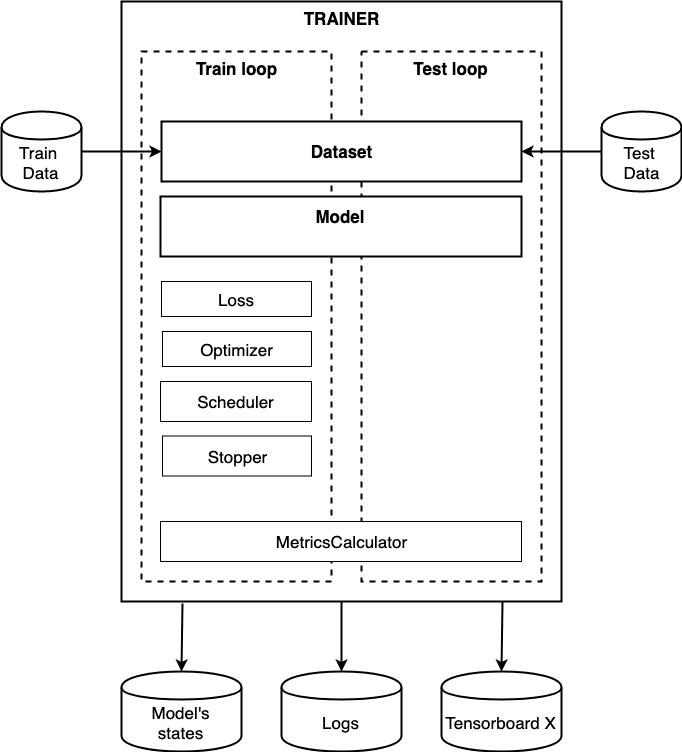
\includegraphics[width=0.95\linewidth]{Programm}
   	\end{center}
   	\caption{Структура программы для тренировки и обучения модели.}
   	\label{tikzpicture: programm}
\end{figure}


\subsection{Выбор метрики}

\indent
\indent
Прежде всего необходимо определиться, как количественно будет оцениваться
точность модели.Мы случайно выбрали 80\% данных 
для тренировки моделей, и 
20\% для их тестирования. В качестве метрик будем использовать 
классические для задачи классификации точность
 (\textit{accuracy}, не путать с \textit{precision}) и взвешенную точность:
выражения \ref{eq:accuracy} и \ref{eq:w_accuracy}.


\begin{equation}\label{eq:accuracy}
	   acc(\vec{y^{gt}}, \vec{y}) = \frac{1}{N}\sum_{i=1}^{N} \delta_{y_i^{gt}, y_i}
\end{equation}
где $\vec{y^{gt}}$ --- вектор номеров классов длинной $N$, 
$\vec{y}$ --- вектор предсказанных номеров классов длинной $N$,
$N$ --- количество рассматриваемых примеров,
$\delta$ --- символ Кронекера.

\begin{equation}\label{eq:w_accuracy}
	   acc_w(\vec{y^{gt}}, \vec{y}) = 
	   \frac{1}{C} \sum_{c}
	   \frac{1}{N_c}\sum_{\{i: y_i^{gt}\equiv c\}} \delta_{y_i^{gt}, y_i}
\end{equation}
где $N_c$ --- количество примеров из класса $c$, $C$ --- количество классов.
 

\indent
\indent
Таким образом, чтобы посчитать точность достаточно просто разделить
количество правильных ответов на общее количество ответов. Чтобы посчитать
взвешенную точность, необходимо вычислить точность для каждого класса
в отдельности, а затем усреднить полученные значения. В случае, если распределение
по классам в значительной степени неравномерное, отсутствие такого усреднения
приведет к тому, что значение метрики будет определяться точностью модели на
нескольких наиболее представленных классах. В данной работе мы будем
смотреть на значения обеих вариантов точности, но для принятия
решений о выборе модели приоритетной является взвешенная точность, так как в нашем наборе данных присутствует большой по размеру класс \textit{other}.


\section{Ход экспериментов}

\indent
\indent
Чтобы обучить модель оптимальным образом, сначала проведем серию
легковесных (с вычислительной точки зрения) экспериментов, чтобы определиться 
со значениями основных гиперпараметров. Затем попробуем улучшить целевую метрику
для лучшей модели, полученной на первом шаге.

\indent
\indent
Начнём с топологии нейронной сети. Будем выбирать из трех семейств архитектур:
 \textit{ResNet}, \textit{Inception} и \textit{VGG}; подробнее см. в разделе \ref{section:archs}.
Чтобы ускорить эксперименты уменьшим размер всех изображений до
$256 \times 256$ пикселей и не будем использовать аугментации во время тренировки.
Прекратим обучение, если в течении 5-ти последних 
эпох\footnote{\textit{Эпохой} в машинном обучении называется один полный проход по
обучающему набору данных в процессе тренировки.} 
не будет улучшено 
значение метрики хотя бы на 0.5\%. В качестве функции потерь используется перекрестная
энтропия (см. раздел \ref{section: losses}), а в качестве оптимизатора параметров 
нейронной сети --- \textit{Adam} \cite{adam}. Кроме того, отследим время, которое 
понадобилось на обучение модели до остановки по названному выше критерию 
\ref{tabular: arch_compare}.


\begin{table}[h]
    \begin{center}
        \begin{tabular}{c | c| c | c | c}
            \hline
            № & Архитектура & Точность & Взвешенная точность  & Время [мин] \\
            \hline
    
            1 & Inception & 0.743 & 0.667 & 239 \\
            
            2 & VGG 11 & 0.678 & 0.565 & 154 \\
            
            3 & VGG 13 & 0.637 & 0.478 & 450 \\
            
            4 & ResNet 18 & 0.692 & 0.602 & 35 \\
            
            5 & ResNet 34 & 0.703 & 0.634 & 119 \\
            
            5 & ResNet 50 & 0.659 & 0.593 & 114 \\
    
            \hline
        \end{tabular}
    \end{center}
    \caption{Сравнение метрик для различных архитектур.}
    \label{tabular: arch_compare}
\end{table}


УЛУЧШЕНИЯ

В процессе тестирования сети применялась техника 
\textit{(TTA Test Time Augmentations)}. Её смысл заключается в том, что на
стадии инференса изображение несколько раз копируется, и к копиям 
применяются аугментации, например, повороты, зеркальные отражения,
изменение контраста и т.д. После чего модель делает предсказание для каждой
копии, а в качестве окончательного ответа вычисляется, например, среднее значение.
Для большинства задач таким образом удается улучшить точность, но сложность
вычислений линейно увеличивается с количеством примененных аугментаций.
Поэтому тодо


\subsection{Полученные результаты}
Картинка с борды, графики метрик, confusion matrix todo



\subsection{Обсуждение результатов}
todo

